\documentclass[]{assignment}

\newcommand{\hwname}{Anirudha Kulkarni}
\newcommand{\hwemail}{2019CS50421}
\newcommand{\hwtype}{Assignment}
\newcommand{\hwnum}{1}
\newcommand{\hwclass}{COL334: Computer Networks}


\begin{document}
\maketitle
\question*{Networking Tools}
    \begin{alphaparts}
        \questionpart IP address of the machine changes with different routers. Each router assigns a private IP address to each device to recognize it between systems connected to network, which can be different. 
            \begin{enumerate}
                \item IP Address with Airtel router: 192.168.1.101
                \item IP Address with BSNL router: 192.168.1.12 
                \item IP Address with Jio mobile hotspot: 192.168.43.179
            \end{enumerate}
        \questionpart 
            \begin{enumerate}
                \item IP address of www.google.com with google dns (8.8.8.8) : 142.250.182.206
                \item IP address of www.facebook.com with google dns (8.8.8.8) : 157.240.1.35  
                \item IP address of www.google.com with multiplay.bsnl.in (218.248.114.1) : 216.58.221.46 
                \item IP address of www.facebook.com with multiplay.bsnl.in (218.248.114.1) : 31.13.79.35 
                \item IP address of www.google.com with cisco OpenDNS (208.67.222.222) : 142.250.66.14 
                \item IP address of www.facebook.com with cisco OpenDNS (208.67.222.222) : 31.13.79.35 
            \end{enumerate}

        \questionpart TTL limits the number of hops a packet can cross. Lower values gives time to live exceeded error as the packet can not reach the destination in limited hops. Received packets have fixed TTL values as it is the response from server. Actual packet size include 8 bytes for ICMP packet header and 20 bytes for IP header. 
            \begin{enumerate} 
                \item Max size for www.iitd.ac.in: 1472 bytes (1500 bytes total)
                \item Max size for www.google.com: 68 bytes (96 bytes total)
                \item Max size for www.facebook.com: 1472 bytes (1500 bytes total)
            \end{enumerate}
            
        Pinging with different values of TTL gives information about the path taken by packet to the destination. Packets with less TTL values expire in the transit exposing the intermediate IP addresses. Ping to www.iitd.ac.in expire till TTL=18. It requires 19 hops to reach the destination.
        \begin{figure}[hbt!]
        \centering
        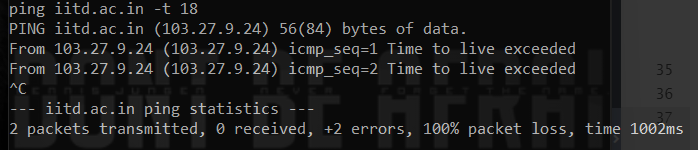
\includegraphics[width=10cm]{assignment-1/report/smallping.png}
        \caption{TTL = 18 packet expires before reaching destination}
        \label{fig:galaxy}
        \end{figure}
        
        \begin{figure}[hbt!]
        \centering
        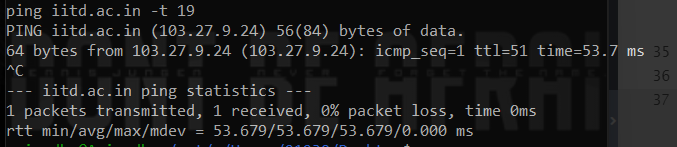
\includegraphics[width=10cm]{assignment-1/report/largeping.png}
        \caption{TTL = 19 packet reaches destination}
        \label{fig:galaxy}
        \end{figure}
        \pagebreak
        \questionpart
        Observations: 
            \begin{enumerate} 
                \item UDP based traceroute generally require large number of hops before reaching to destination as most of the routers do not reply to UDP protocol as it is unreliable protocol. The Internet Control Message Protocol (ICMP) is a network layer protocol used by network devices to diagnose network communication issues which is default in Windows. Linux, by default, uses UDP.     
                \begin{figure}[hbt!]
                \centering
                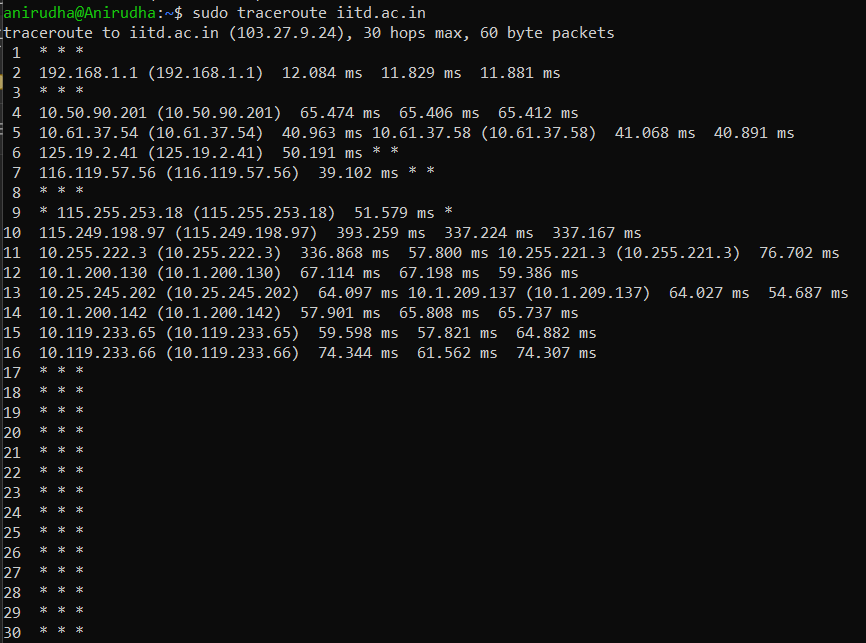
\includegraphics[width=16cm]{assignment-1/report/udpping.png}
                \caption{UDP traceroute - many servers did not reply}
                \label{fig:galaxy}
                \end{figure}
                
                \begin{figure}[hbt!]
                \centering
                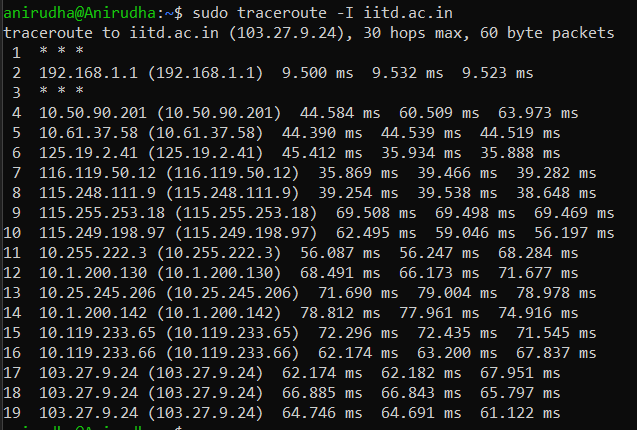
\includegraphics[width=10cm]{assignment-1/report/icmpping.png}
                \caption{ICMP traceroute}
                \label{fig:galaxy}
                \end{figure}
                \item -I parameter in Linux can make traceroute to send ICMP packets
                \item Some paths by default use IPv6 and can be made to use IPv4 with -4 argument. This works only when resolving a host name returns both IPv4 and IPv6 addresses. Similarly -6 forces to use IPv6.
                
                
             \end{enumerate}
    \end{alphaparts}
    \pagebreak
    
\question*{Packet Analysis}
Corresponding wire-shark snapshot is attached with the zip file. 
\begin{alphaparts}
    \questionpart DNS request took 1.686420000 - 1.679274000 = 0.007146 sec = 7.146 milliseconds.
    \begin{figure}[hbt!]
    \centering
    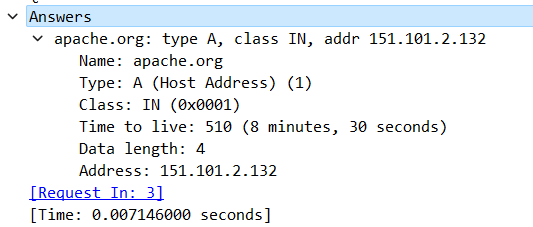
\includegraphics[width=8cm]{assignment-1/report/dnstime.png}
    \caption{DNS request response}
    \label{fig:galaxy}
    \end{figure}
    \questionpart Approximately 28 http requests were generated. Most of the initial requests (25) are made to 151.101.2.232 which is IP address of the http://apache.org. These requests fetch the HTML content then CSS for styling, images and javascript for dynamic behaviour. Towards the end HTTP requests are made to 172.217.166.238 for google search optimization and 142.250.77.238 for advertisements on the website.
    \begin{figure}[hbt!]
    \centering
    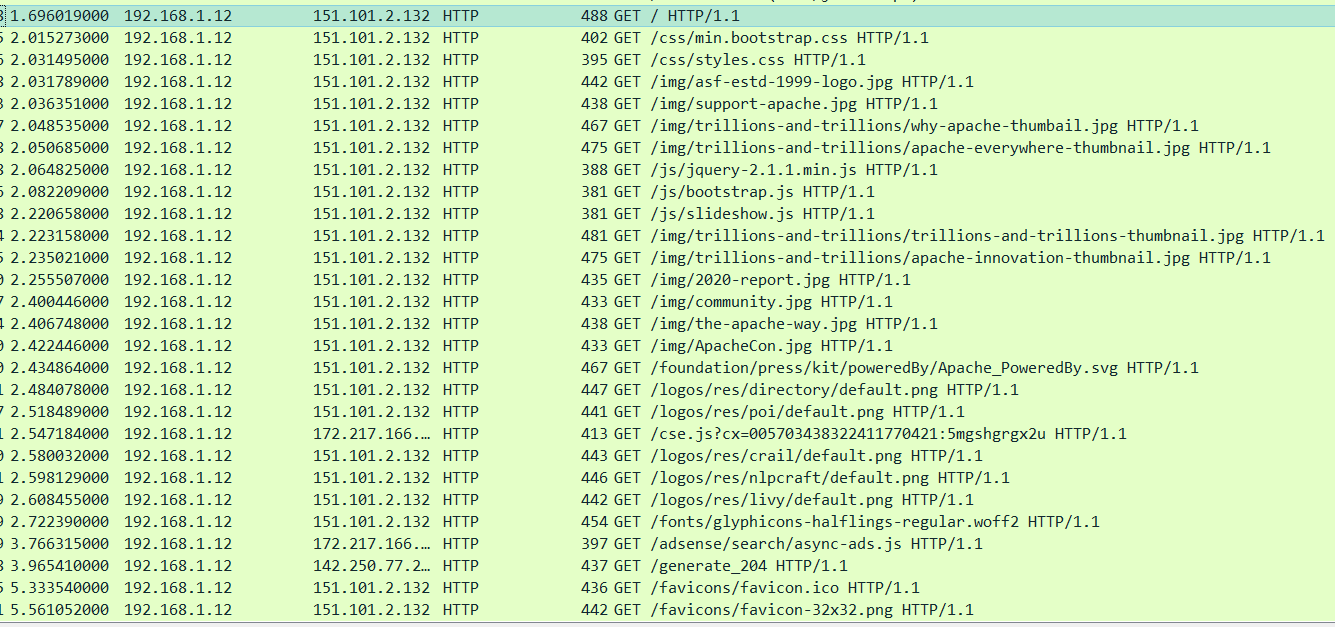
\includegraphics[width=15cm]{assignment-1/report/getrequests.png}
    \caption{HTTP requests}
    \label{fig:galaxy}
    \end{figure}
    \questionpart Last packet (2084th packet) arrival time (including google search manager and advertisement resources) : 5.838546000 sec. Total time taken = 5.838546000 - 1.679274000 = 4.159272 seconds.
    \questionpart There is only 1 request and corresponding response via HTTP protocol. GET request to http://www.cse.iitd.ac.in was responded with 301 response i.e. web-page moved permanently to https://www.cse.iitd.ac.in which uses HTTPS protocol. HTTPS traffic is encrypted using TLS protocol and hence can not be intercepted in clear text. The encrypted data shared can be filtered with TLS filter.
            \begin{figure}[hbt!]
    \centering
    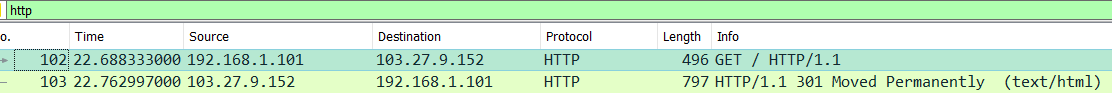
\includegraphics[width=14cm]{assignment-1/report/moved.png}
    \caption{Permanently moved response}
    \label{fig:galaxy}
    \end{figure}

 \end{alphaparts}
   \pagebreak
    
\question*{Implement Traceroute using Ping}
Traceroute involves following steps:

\begin{enumerate}
    \item initialize t=1
    \item ping destination with ttl=t and get the IP address at which the Time To Live exceeded message appears. This is the hop where packet expired.
    \item ping the IP address from (2) with a large TTL (say 50) to get RTT for the IP.
    \item repeat 2-3 with t=t+1 until the destination is reached.
    \item repeat 1-2-3-4 steps 3 times to remove any bias or alternate path taken by the packet.
 \end{enumerate}
    Traceroute implementation with ping command in python hop by hop
        \begin{figure}[hbt!]
    \centering
    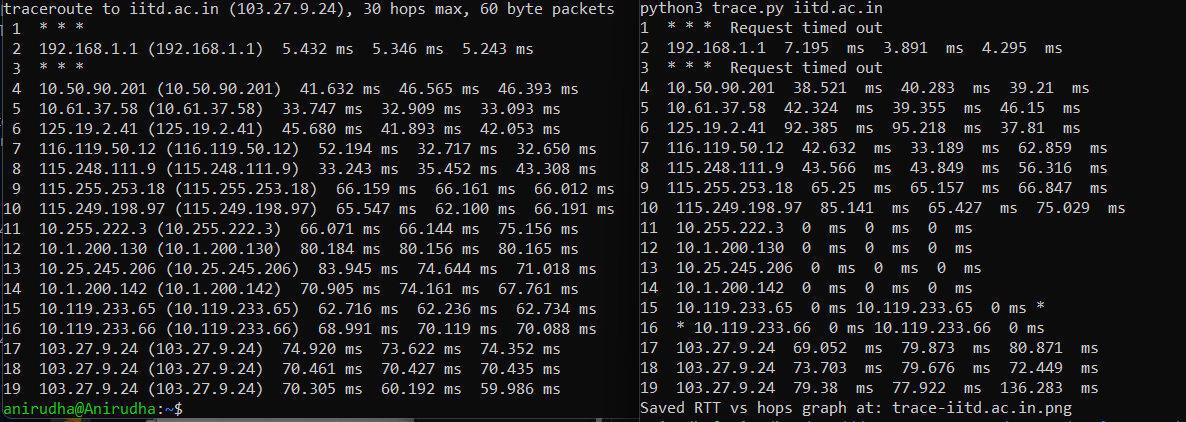
\includegraphics[width=18cm]{assignment-1/report/graph.png}
    \caption{traceroute command for iitd.ac.in (left) vs custom code (right)}
    \label{fig:galaxy}
    \end{figure}
        \begin{figure}[hbt!]
    \centering
    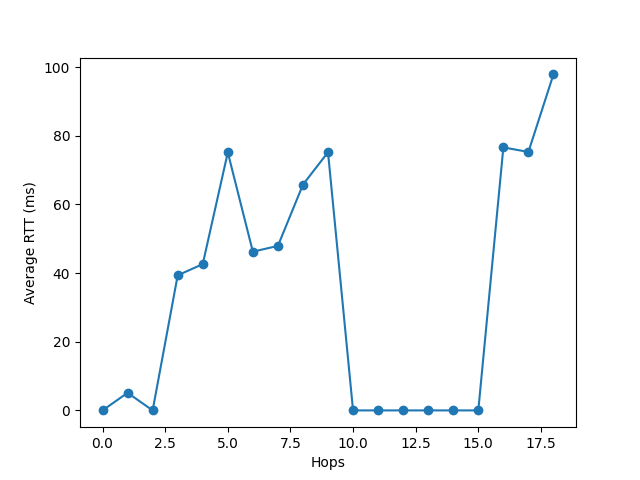
\includegraphics[width=10cm]{assignment-1/report/trace-iitd.ac.in.png}
    \caption{RTT vs Hops graph for iitd.ac.in (servers that did not respond to ping are marked with 0 RTT)}
    \label{fig:galaxy}
    \end{figure}
            \begin{figure}[hbt!]
    \centering
    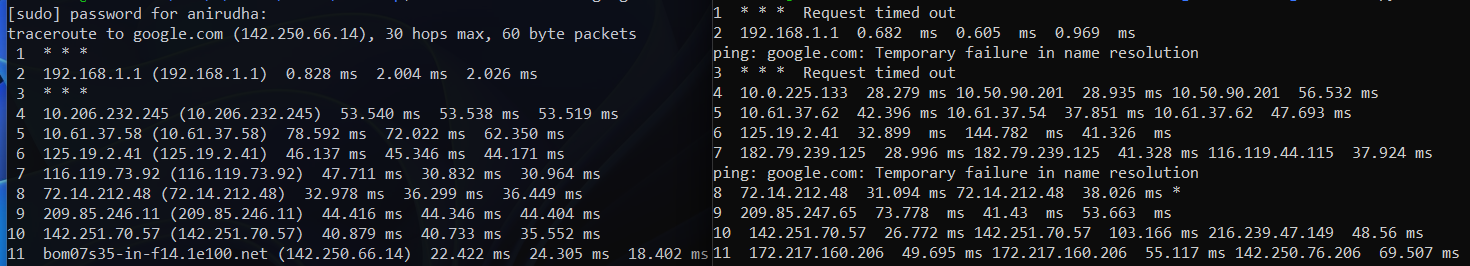
\includegraphics[width=18cm]{assignment-1/report/googleping.png}
    \caption{traceroute command for google.com (left) vs custom code (right)}
    \label{fig:galaxy}
    \end{figure}
        \begin{figure}[hbt!]
    \centering
    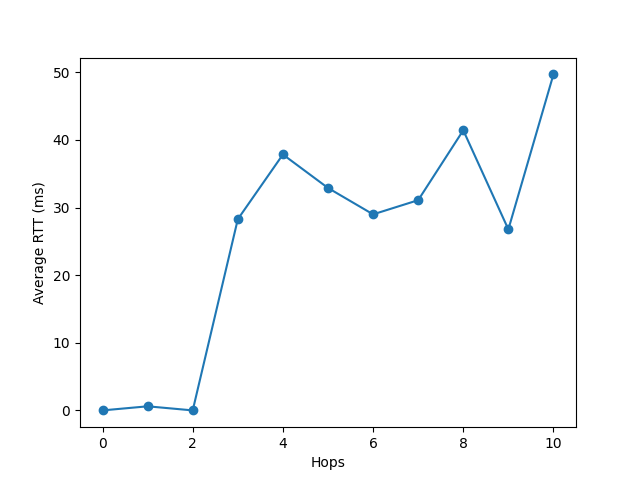
\includegraphics[width=6cm]{assignment-1/report/trace-google.com.png}
    \caption{RTT vs Hops graph for google.com (servers that did not respond to ping are marked with 0 RTT)}
    \label{fig:galaxy}
    \end{figure}
                \begin{figure}[hbt!]
    \centering
    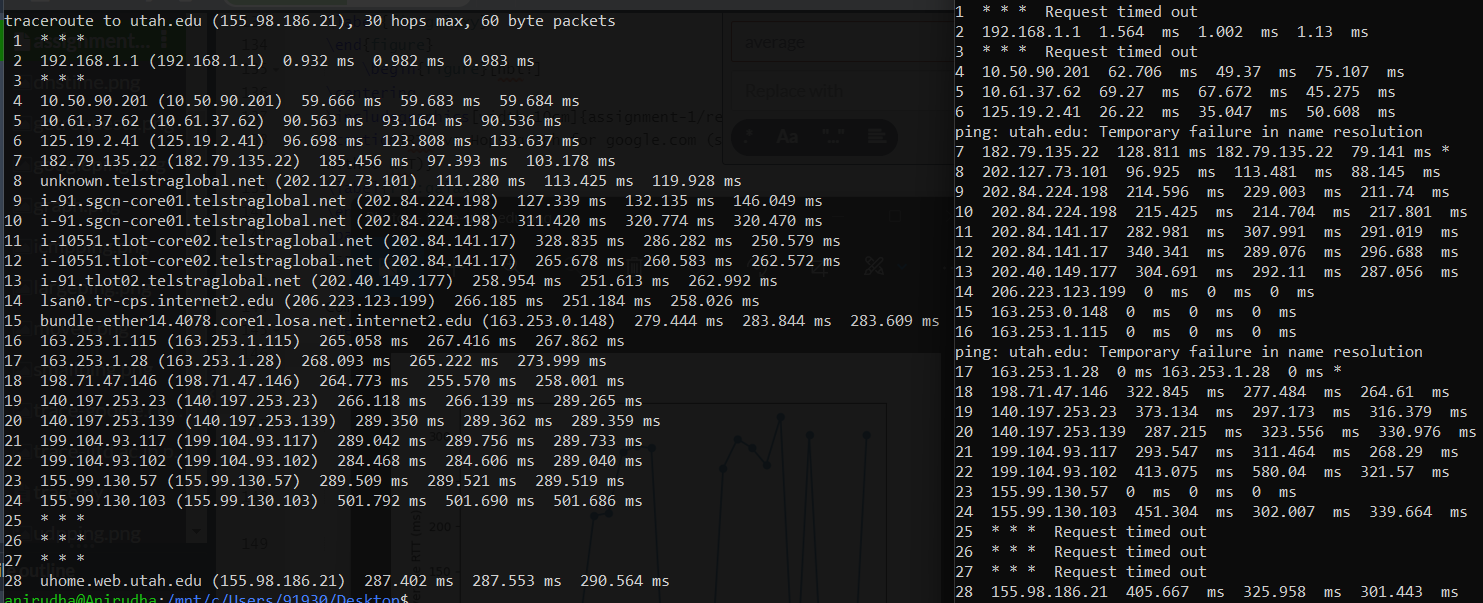
\includegraphics[width=18cm]{assignment-1/report/utah.png}
    \caption{traceroute command for utah.edu (left) vs custom code (right)}
    \label{fig:galaxy}
    \end{figure}
        \begin{figure}[hbt!]
    \centering
    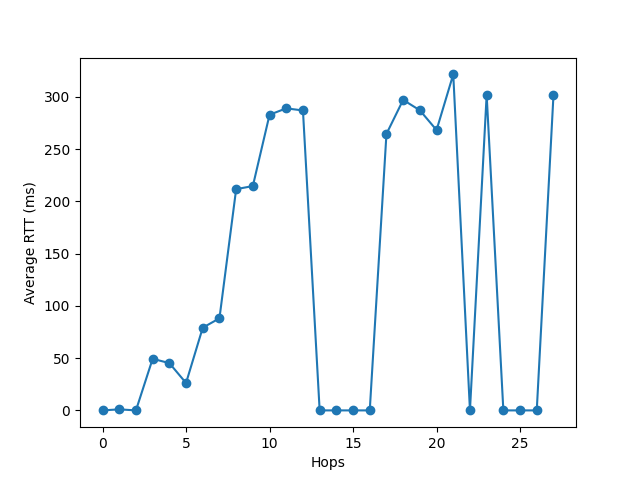
\includegraphics[width=7cm]{assignment-1/report/trace-utah.edu.png}
    \caption{RTT vs Hops graph for utah.edu (servers that did not respond to ping are marked with 0 RTT)}
    \label{fig:galaxy}
    \end{figure}
    \pagebreak
    Usage: python3 trace.py <domain>
    \\
    Complexity vs Efficiency trade-off:
    \begin{enumerate}
        \item RTT of some intermediate servers is more noisy due to variation of load in routers. This can be removed by sending multiple packets across each iteration and taking minimum.
        \item Currently default is minimum of 3 path each sending 2 packets. This can be changed in the program. Sending 3 packets in each iterations severely affects the complexity causing time to shoot up to 2 minutes
        \item Sending single packet at 3 paths gives lot of noise and graph is difficult to make any inferences. Hence we choose 2 packets at 3 paths to get most optimal solution
        \item Time complexity is further reduced by adding timeout of 1 seconds to reduce time spent in waiting for servers to respond that are not responding. The maximum RTT observed was less than 500ms hence giving 1 second timeout safely reduces the time by a significant factor.
    \end{enumerate}
    \lstinputlisting[language=python,caption=Python implementation for traceroute using ping]{trace.py}

\listoffigures
\lstlistoflistings



\end{document}
